\documentclass[12pt, legalpaper]{article}

\usepackage{graphicx}
\usepackage{cleveref}
\usepackage{parskip}
\usepackage{rotating}
\usepackage{tabularx}
\usepackage{tikz}
\usepackage{graphicx}
\usepackage{rotating}
\usepackage[
backend=biber,
style=apa,
]{biblatex}

\addbibresource{ref.bib}

\graphicspath{images/}

\def\checkmark{\tikz\fill[scale=0.4](0,.35) -- (.25,0) -- (1,.7) -- (.25,.15) -- cycle;}

\graphicspath{{images/}}


\title{Documentatie: Robotarm simulatie}
\author{Mart Rietdijk (1673342)}
\date{24 oktober 2023}


\begin{document}
    \begin{titlepage}
        \maketitle
        \begin{center}
            Klas: ITN-WOR-A-s

            Docent: Jorg Visch

            Course: Wor World

            Versie: 1.0
        \end{center}
        \thispagestyle{empty}
    \end{titlepage}
    \tableofcontents
    \newpage

    \section{Inleiding}
    Er zijn veel redenen om hardware in de daadwerkelijke wereld te simuleren.
    Daarom is deze simulatie opgezet om de meeste risico's van het werken met een robotarm af te vangen.

    In dit document is te vinden hoe de simulatie-opdracht is uitgewerkt.

    \section{De Requirements}
    \begin{table}[h]
        \begin{tabularx}{1\textwidth} {|c|X|c|c|}
            \hline
            \textbf{ID} & \textbf{Wat is er gedaan?} & \textbf{Prio} & \textbf{Klaar?}\\
            \hline\hline
            PA01 & Alle code is gepackaged volgens de ROS-directorystructuur. & Should & \checkmark \\
            \hline
            PA02 & Package is te bouwen met colcon op ROS2 Humble Hawksbill & Must & \checkmark \\
            \hline
            PA03 & De applicatie wordt gebouwd met C++ volgens de Object Oriented principes die je geleerd hebt bij eerdere courses. & Must & \checkmark \\
            \hline
            PA04 &  & Should & $\times$ \\
            \hline
        \end{tabularx}
        \caption{Requirements tabel}
        \label{tab:reqpa}
    \end{table}

    \begin{table}[h]
        \begin{tabularx}{1\textwidth} {|c|X|c|c|}
            \hline
            \textbf{ID} & \textbf{Wat is er gedaan?} & \textbf{Prio} & \textbf{Klaar?}\\
            \hline\hline
            VS01 & De virtuele controller luistert naar een topic waarop string messages in het formaat van de SSC-32U 1 worden geplaatst. Van de interface moeten ten minste commando's zijn opgenomen voor het verplaatsen van de servo's met een ingestelde duur en het stoppen van de servo's. & Must & \checkmark \\
            \hline
            VS02 & De virtuele controller reageert op het topic (zie eis VS01) door bijbehorende joint\_state messages te publiceren. & Must & \checkmark \\
            \hline
            VS03 & De virtuele robotarm wordt gevisualiseerd in Rviz (een URDF-model van de arm is beschikbaar op OnderwijsOnline). & Must* & \checkmark \\
            \hline
            VS04 & De virtuele robotarm gedraagt zich realistisch m.b.t. tijdgedrag (servo's roteren kost tijd en gaat geleidelijk). & Must & \checkmark \\
            \hline
            VS05 &  & Should & $\times$ \\
            \hline
        \end{tabularx}
        \caption{Requirements tabel}
        \label{tab:reqvs}
    \end{table}

    \begin{table}[h]
        \begin{tabularx}{1\textwidth} {|c|X|c|c|}
            \hline
            \textbf{ID} & \textbf{Wat is er gedaan?} & \textbf{Prio} & \textbf{Klaar?}\\
            \hline\hline
            VC01 & & Should & $\times$ \\
            \hline
            VC02 & Publiceert een 3D-visualisatie van het bekertje voor Rviz. & Must* & \checkmark \\
            \hline
            VC03 &  & Should & $\times$ \\
            \hline
            VC04 & & Could* & $\times$ \\
            \hline
            VC05 & & Should & $\times$ \\
            \hline
            VC06 & Het bekertje beweegt mee met de gripper (als hij vastgehouden wordt). & Must & \checkmark \\
            \hline
            VC07 & Bekertje is onderhevig aan zwaartekracht wanneer losgelaten. & Must & \checkmark \\
            \hline
            VC08 & Bekertje bepaalt en publiceert zijn positie. & Must & \checkmark \\
            \hline
            VC09 & Bekertje bepaalt en publiceert zijn snelheid. & Should & $\times$ \\
            \hline

        \end{tabularx}
        \caption{Requirements tabel}
        \label{tab:reqvc}
    \end{table}

    \newpage

    \begin{table}[h]
        \begin{tabularx}{1\textwidth} {|c|X|c|c|}
            \hline
            \textbf{ID} & \textbf{Wat is er gedaan?} & \textbf{Prio} & \textbf{Klaar?}\\
            \hline\hline
            DI01 & Een demoscript stuurt over de tijd een sequentie van commando's naar de armcontroller. 2 & Must & \checkmark \\
            \hline
            DI02 & & Could & $\times$ \\
            \hline
            DI03 & & Could & $\times$ \\
            \hline


        \end{tabularx}
        \caption{Requirements tabel}
        \label{tab:reqdi}
    \end{table}

    \begin{table}[h]
        \begin{tabularx}{1\textwidth} {|c|X|c|c|}
            \hline
            \textbf{ID} & \textbf{Wat is er gedaan?} & \textbf{Prio} & \textbf{Klaar?}\\
            \hline\hline
            DM01 & Beschrijft hoe de code gebouwd kan worden. & Must & \checkmark \\
            \hline
            DM02 & Beschrijft stap voor stap hoe de arm bewogen kan worden middels enkele voorbeelden. & Must & \checkmark \\
            \hline
            DM03 & Beschrijft welke eisen gerealiseerd zijn. En geeft hierbij een (korte) toelichting. & Must & \checkmark \\
            \hline
        \end{tabularx}
        \caption{Requirements tabel}
        \label{tab:reqvc}
    \end{table}

    \begin{table}[h]
        \begin{tabularx}{1\textwidth} {|c|X|c|c|}
            \hline
            \textbf{ID} & \textbf{Wat is er gedaan?} & \textbf{Prio} & \textbf{Klaar?}\\
            \hline\hline
            DD01 & Beschrijft de structuur van de package (Nodes, topics, messages, et cetera). & Must & \checkmark \\
            \hline
            DD02 & Beschrijft de structuur en samenhang van de broncode (class-diagrams, beschrijving, et cetera). & Must & \checkmark \\
            \hline
            DD03 &  & Could & $\times$ \\
            \hline
            DD04 & De API is beschreven in Hoofdstuk Commando's & Should & \checkmark \\
            \hline
        \end{tabularx}
        \caption{Requirements tabel}
        \label{tab:reqdd}
    \end{table}

    \newpage
    
    \section{ROS-structuur}
    In ROS is een structuur te beschrijven in Topic, services, Nodes, en Actions.
    Deze structuur wordt in dit hoofdstuk besproken per ROS-package.
    De structuur is te vinden in het onderstaande plaatje (\cref{fig:full-structure}).
    \subsection{Console package}
    De Console package published een Node ``Console''.
    Deze Node published weer een Topic command. Deze Topic is van het type Command beschreven in de package robot\_arm\_interface.
    Deze Topic bevat een string. Deze wordt gevraagd door de Node ``Console'' en verstuurd via deze Topic naar de Node robot\_arm\_interface.

    \subsection{Simulation package}
    In De Simulation package worden de volgende Nodes gepublished (met een kleine beschrijving):
    \begin{itemize}
        \item robot\_arm\_publisher: Published alle joints van de robotarm
        \item robot\_publisher: Is de standaard robot\_state\_publisher van ROS2
        \item cup\_picked\_up: Is een tf listener die kijkt of dat de arm de cup vast heeft
        \item cup\_publisher: Published de cup frame
    \end{itemize}
    Deze Nodes bieden hun eigen Topics weer aan (met een kleine beschrijving):
    \begin{itemize}
        \item joint\_states: De Topic die de status van de joints van de robotarm published
        \item picked\_up\_cup: De Topic die aangeeft of de cup wordt opgepakt door de robotarm
        \item robot\_description: De Topic die de robotarm URDF aan RViz geeft
        \item cup\_description: De Topic die de cup URDF aan RViz geeft
    \end{itemize}

    \subsubsection{Robotarm}
    De robot\_arm\_publisher aanvaardt het commando op het Topic command, en leest dit uit met de parser.
    Het commando dat op command wordt gepublished kan een commando zijn die zegt op welke PWM waarde de servo moet staan en hoe lang hij hier over mag doen, of een commando om alle servo's die bewegen te stoppen.
    De commando's komen in hoofdstuk \ref{commands} aan bod.

    In de launchfile wordt de URDF aan de robot\_arm\_interface meegegeven. Daaruit leest de Node de URDF in en published de joint states naar de Topic joint\_states.

    Deze joint states worden opgevangen door de robot\_publisher Node. Deze Node verwerkt de states en published op basis daarvan de frames naar het tf framework.

    \subsubsection{Cup}
    Naast de robotarm staat er ook een bekertje (cup) in de wereld.
    Daarvoor zorgt de cup\_publisher Node. Deze published een cup frame naar het tf framework.
    Deze cup frame heeft een afstand ten opzichte van de robotarm. 
    
    De cup\_publisher luistert naar de Topic picked\_up\_cup. Op deze Topic wordt of de afstand van de cup naar de onderkant van de robotarm gestuurd, of de afstand van de cup ten opzichte van de hand.
    Deze keuze wordt gebaseerd op het feit dat de robotarm de cup vast heeft of niet.
    Dit is te meten aan de afstand van de grippers van de robotarm ten opichte van de cup.
    
    Als de robotarm de cup vast heeft, wordt de afstand van de hand gestuurd, en houdt de cup deze afstanden vast.
    En als de robotarm de cup niet vast heeft, valt de cup op de grond ten opzichte van de onderkant van de robotarm.

    \subsubsection{RViz}
    Op de Topics cup\_description en robot\_description, worden de URDFs van de robotarm en cup gepublished als string.
    Dit wordt gedaan zodat RViz weet bij welke joint wat te tekenen.


    \begin{sidewaysfigure}
        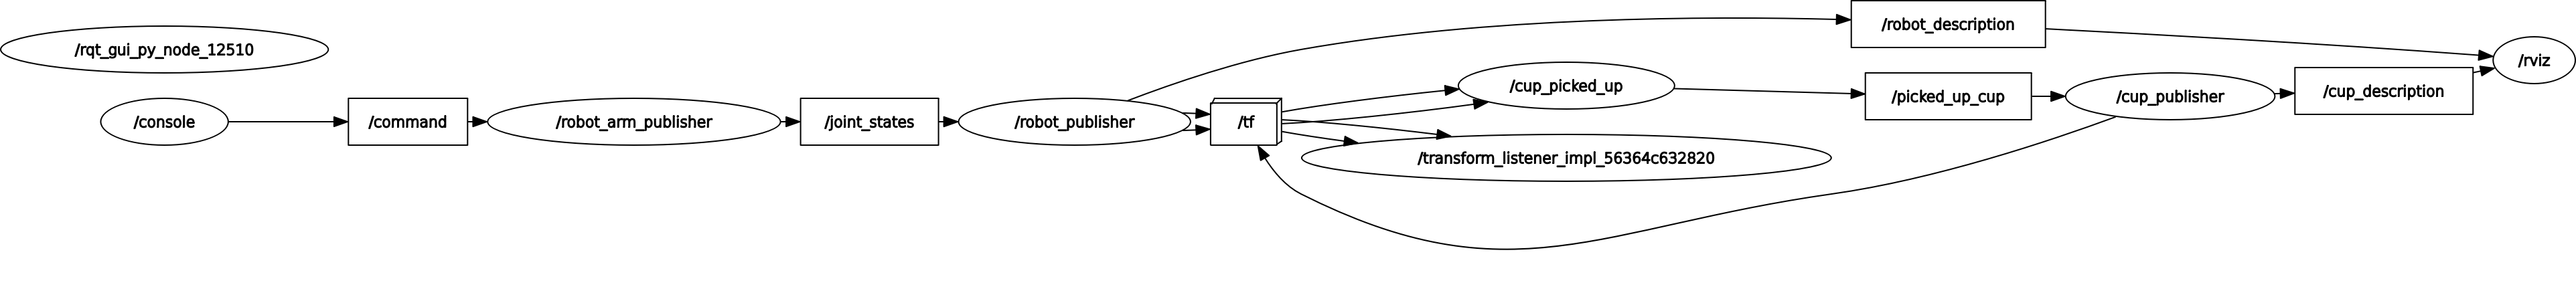
\includegraphics[width=1\textwidth]{rosgraph}
        \caption{Volledige ROS-structuur}
        \label{fig:full-structure}
    \end{sidewaysfigure}

    \newpage

    \section{Klassendiagram}
    In dit hoofdstuk wordt het klassendiagram van de applicatie besproken.
    Het klassen diagram is te zien in afbeelding \cref{fig:classdiagram}.
    Hieronder volgt een beschrijving per klasse.

    \subsection{RobotArmJointPublisher}
    In deze klasse wordt de URDF van de robot-arm ingeladen. Van de URDF worden de joints opgeslagen in een map ``joints''.
    Deze map bestaat uit de joint naam en de huidige positie van de joint.
    Nadat de joints worden aangemaakt worden deze om de 10 milliseconden gepublished. Dit wordt gedaan door de functie publishJointStates.
    
    Wanneer een commando binnenkomt op de commandSub wordt de commandCallback methode aangeroepen. Daarna worden de PWM waarden van het commando omgerekend tot radialen.
    Daarna worden er stappen in radialen per milliseconden berekend.
    Deze stappen worden doorgegeven aan de sendJointToPos methode. Deze methode maakt een thread aan die voor het aantal milliseconden dat het commando aangeeft, de stappen bij de huidige positie worden opgeteld.
    Deze thread wordt opgeslagen in de movingThreads vector, zodat als er een stop commando wordt gegeven de thread nog gestopt kan worden.

    Als er een commando ``STOP'' binnenkomt, worden de opgeslagen threads in de vector direct gestopt.

    \subsection{CupStatePublisher}
    In CupStatePublisher wordt eerst de URDF ingeladen met behulp van setupUrdf.
    Deze URDF wordt daarna op zijn tijd gepublished d.m.v. de methode publishCup.

    De CupStatePublisher heeft ook een subscription op een Topic waar de postie ten opzichte van de hand of onderkant van de robotarm wordt geplublished.
    Op basis daarvan zorgt de methode updatePos of de positie van de cup beweegt of niet.

    \subsection{PickedUpCupListener}
    De PickedUpCupListener kijkt of de gripper de cup vast heeft ja of nee. Daar op basis geeft hij de afstand van de hand of de afstand van de onderkant van de robotarm.
    Dit doet hij in de functie timerCallback, die om de 100 milliseconden op de topic published.

    \subsection{Parser}
    Omdat er commando's in string formaat komen, in de vorm van een protocol van Lynxmotion SSC-32U USB Servo Controller Board (\cite{lynxmoti36:online}), moet er een Parser aan boord zijn van de RobotArmJointPublisher.
    Deze Parser maakt op basis van een statemachine bekend wat de servonr, pwm, en tijd is per bericht.
    Dit gebeurt door een Parser object aan te maken met een string. Direct in de constructor parsed hij het bericht.
    Door middel van de getters kunnen deze waarden opgehaald worden. Dit gebeurt dus ook per commando in RobotArmJointPublisher.

    Naast een commando voor het bewegen van een servo, kan er ook een stop commando geparsed worden.

    \begin{sidewaysfigure}
        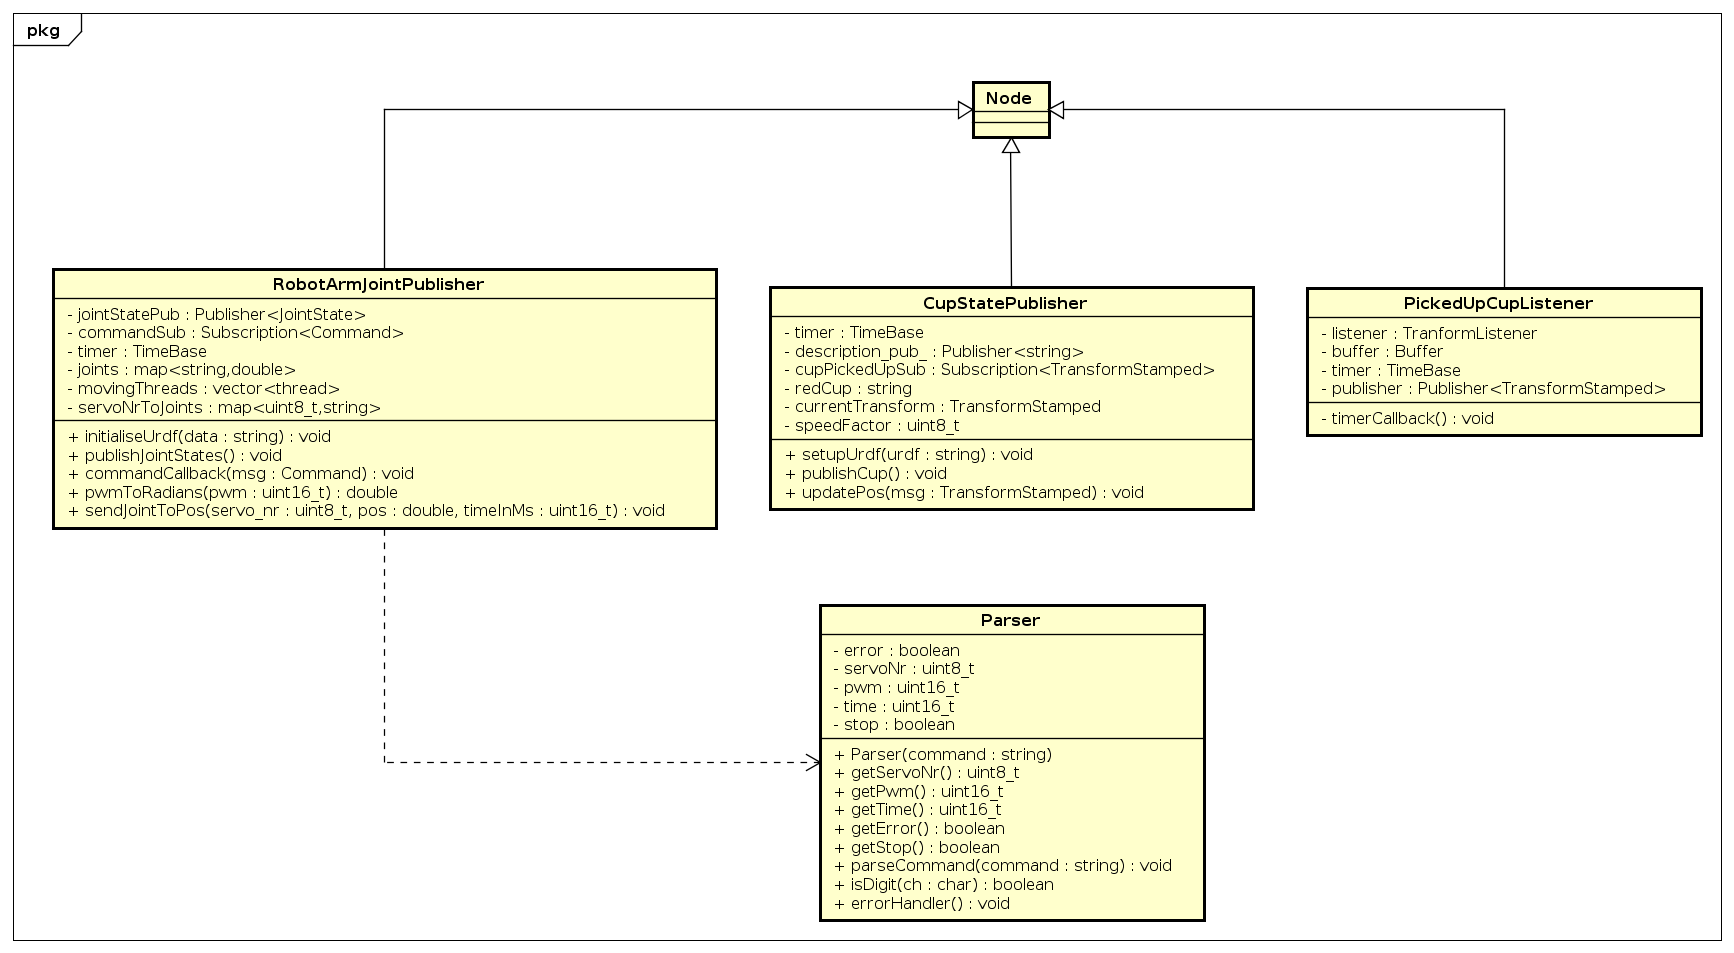
\includegraphics[width=1\textwidth]{KlassenDiagramSimulation}
        \caption{Klassendiagram simulation}
        \label{fig:classdiagram}
    \end{sidewaysfigure}

    \newpage

    \section{Robot-commando's}
    \label{commands}
    In het volgende tabel staan de commando's die gestuurd kunnen worden naar de robotarm.
    Deze commando's komen voort uit de SSC-32u protocol beschrijving (\cite{lynxmoti36:online})

    \begin{table}[h]
        \begin{tabularx}{1\textwidth} {|c|X|}
            \hline
            \textbf{Commando} & \textbf{Beschrijving}\\
            \hline\hline
            $\#\langle servoNr\rangle P\langle pwm \rangle T\langle time In Ms \rangle$\textbackslash r & Beweegt een servo naar de aangegeven PWM. Dit duurt het aantal aangegeven milliseconden. De minimale waarde voor pwm is 1000 en maximale waarde is 2000.\\
            \hline
            STOP & Stopt alle bewegende servo's\\
            \hline
        \end{tabularx}
        \caption{Commando's tabel}
        \label{tab:commands}
    \end{table}

    \printbibliography
    
\end{document}